\chapter{Introduction}

Improving inference of fundamental stellar properties such as age, mass and radius is important for improving our understand of the chronology of the Milky Way and measuring the properties of exoplanets. In the last few years, asteroseismology has been able to provide tighter constraints on stellar properties [CITE]. However, as we reduce our precision, the systematic uncertainties from our choice of model physics begin to dominate. We need a way to model additional physics without sacrificing precision and to account for the effects of extra stellar physics.

In this report, I will first introduce a new method for determining stellar parameters through the use of a hierarachical Bayesian model (HBM). Then, I will explain how we predict observables from stellar evolutionary codes. In Section \ref{sec:seismo} I introduce asteroseismology and show how the detection of stellar oscillations can probe the structure of a star. I then explain how we sample from our models of stellar evolution and asteroseismology, introducing the need for machine learning to speed-up the process and increase the scalability of the HBM. Once we have a way of making predictions of observables, I describe how we measure such properties in stars.

In Chapter \ref{ch:paper} I will introduce my paper which applies the methods in this chapter to a sample of stars with asteroseismic detections already studied by \citet{Serenelli.Johnson.ea2017}. I will show that, with the assistance of machine learning, we can reduce statistical uncertainties on ages, masses and radii to $\sim 10\%$, $\sim 3\%$ and $\sim 1\%$ respectively, despite increasing the number of free parameters in the model over what is currently done in the literature.

Finally, in Chapter \ref{ch:future} I will propose an extension to the method whisch introduces a new observable to improve the inference of helium abundance in stars.

\section{Hierarchical Bayesian Models}\label{sec:hbm}

In this section, I begin by describing a Bayesian probabilistic model of a star. Then, I show how we can extend the model to an HBM which introduces parameters to describe a population of stars. I demonstrate, with a simple example, that such a method can improve the inference of fundamental parameters.

Consider a model for a single star comprising a set of independent parameters, $\bm{\theta} = \{\theta_i\}_{i=1}^{N_\theta}$ which makes a set of predictions, $\bm{\mu} = \bm{f} (\bm{\theta})$, where $\bm{\mu} = \{\mu_{j}\}_{j=1}^{N_y}$ and $N_y$ is the number of observables. Using Bayes' theorem, we may write the \emph{posterior} probability density function (PDF) of the model given a set of observations $\bm{y}$ as,
%
\begin{equation}
    p(\bm{\theta}|\bm{y}) \propto p(\bm{y}|\bm{\theta})\,p(\bm{\theta}),
    \label{eq:bayes}
\end{equation}
%
where $p(\bm{y}|\bm{\theta})$ is the \emph{likelihood} of the data given the model and $p(\bm{\theta})$ is the \emph{a priori} PDF of the model parameters.

Assuming our observations of $\bm{y}$ are uncorrelated and subjected to random, Gaussian noise with a known standard deviation, $\bm{\sigma}_y$, we may write the likelihood function as a normal distribution,
%
\begin{align}
    p(\bm{y}|\bm{\theta}) = &\prod_{j=1}^{N_y} \frac{1}{\sigma_{y,\,j} \sqrt{2\pi}} \exp \left[ - \frac{(y_j - \mu_{y,\,j})^2}{2 \sigma_{y,\,j}^2} \right],\\
    \equiv &\prod_{j=1}^{N_y} \mathcal{N}(y_j | \mu_{y,\,j}, \sigma_{y,\,j}),
\end{align}
%
where $\mathcal{N}(x | \mu, \sigma)$ is a normal distribution for $x$ with a mean, $\mu$ and standard deviation $\sigma$.

The prior PDF of the model, assuming the parameters are independent, is $p(\bm{\theta}) = \prod_i p(\theta_i)$. Encoding our prior understanding of the model this way is useful for improving our inference. For example, we have independent prior understand that the age of the universe is $\sim \SI{14}{\giga\year}$ [CITE]. Hence, we may choose to give the age parameter for a stellar model a uniform prior PDF from \SIrange{0}{14}{\giga\year} such that our posterior PDF is not influenced by unphysical ages.

Once we have the posterior, we can determine the marginalised posterior distribution of an individual parameter by integrating over all other parameters. For example, the marginalised posterior for $\theta_1$ is,
%
\begin{equation}
    p(\theta_1 | \bm{y}) = \int_{-\infty}^{+\infty} p(\bm{\theta} | \bm{y}) \, \dd \theta_2 \dots \dd \theta_{N_{\theta}}.
\end{equation}
%
Therefore, we end up with a distribution which describes the probability of $\theta_1$ given $\bm{y}$ which takes into account the distribution (or uncertainty) of all other parameters in the model.

Let us now consider modelling a population of $N_\mathrm{obj}$ similar stars. We could combine the posteriors for each star to get a posterior for the population of stars like so,
%
\begin{equation}
    p(\bm{\Theta}|\bm{Y}) = \prod_{k=1}^{N_\mathrm{obj}} p(\bm{\theta}_k|\bm{y}_k),
\end{equation}
%
where $\bm{\Theta} = \{\bm{\theta}_k\}_{k=1}^{N_\mathrm{obj}}$ and $\bm{Y} = \{\bm{y}_k\}_{k=1}^{N_\mathrm{obj}}$ are the matrices of model parameters and observations. We refer to this as a \emph{no-pooled} model because no information is shared between the objects. 

However, what if we have a model which describes the distribution of a particular parameter $\bm{\theta}_i$ in the population? For example, if we have prior knowledge that stars in an stellar cluster have to have formed at roughly the same time, we might want to encode such information into the model. One method would be to independently model the stars in the cluster and then find their mean and standard deviation in age. This method typically over-predicts the standard deviation because it fails to account the individual stellar uncertainties [CITE]. Alternatively, we can incorporate the assumption that stars in a cluster formed at the same time using one of two ways. The first is to \emph{partially-pool} and the second is to \emph{max-pool} the stellar ages respectively. The former assumes the stellar parameters are drawn from some common distribution, and the latter is the special case where all stellar parameters share the same value in the population.

We refer to models which pool parameters in this way as hierarachical models[CITE]. For a hierarchical model, we describe the distribution of $\bm{\Theta}$ in the population by a set of \emph{hyper-parameters}, $\bm{\phi} = \{ \phi_l \}_{l=1}^{N_\phi}$. Bayes' equation now becomes,
%
\begin{equation}
    p(\bm{\phi}, \bm{\Theta} | \bm{Y}) \propto p(\bm{Y} | \bm{\Theta}) \, p(\bm{\Theta} | \bm{\phi}) \, p(\bm{\phi})
\end{equation}
%
where the probability of $\bm{\Theta}$ given $\bm{\phi}$ is,
%
\begin{equation}
    p(\bm{\Theta} | \bm{\phi}) = \prod_{k=1}^{N_\mathrm{obj}} d(\bm{\theta}_k | \bm{\phi}),
\end{equation}
%
and $d(\bm{\theta}_k | \bm{\phi})$ is some chosen distribution from which the parameters for a given star are drawn from the population.

Let us consider a simple model which predicts the luminosities, $\bm{L}$ from the ages, $\bm{\tau}$ of $N_\mathrm{obj} = 1000$ stars in a cluster formed at roughly the same time. Modelling the population independently, we get the posterior,
%
\begin{equation}
    p(\bm{\tau} | \bm{L}) \propto \prod_{k=1}^{1000} p(L_k | \tau_k) \, p(\tau_k).
    \label{eq:age-np}
\end{equation}
%

Now, let us consider a partially-pooled model where the stellar ages are drawn from a normal distribution centred on a mean, $\mu_\tau$ and standard deviation, $\sigma_\tau$. The posterior now becomes,
%
\begin{equation}
    p(\mu_\tau, \sigma_\tau, \bm{\tau} | \bm{L}) \propto p(\bm{L} | \bm{\tau}) \, p(\bm{\tau} | \mu_\tau, \sigma_\tau) \, p(\mu_\tau, \sigma_\tau),
    \label{eq:age-pp}
\end{equation}
%
where,
%
\begin{equation}
    p(\bm{\tau} | \mu_\tau, \sigma_\tau) = \prod_{k=1}^{1000} \mathcal{N}(\tau_k | \mu_\tau, \sigma_\tau).
\end{equation}

There is no known analytical or empirical relation between the age of a star and its luminosity, but for the purposes of this example let us say that we know $L \propto \tau^{2}$. I generated 1000 stellar ages from a normal distribution with a mean of \SI{5}{\giga\year} and a standard deviation of \SI{0.05}{\giga\year}, and computed their luminosities using this relation. Then, I added Gaussian noise to the luminosities with a standard deviation of \SI{0.05}{\solarluminosity} and proceeded to model the stellar ages using Equations \ref{eq:age-np} and \ref{eq:age-pp} and the Bayesian package \texttt{pymc3} [CITE]. The observed and true luminosities are plot against the true ages in Figure \ref{fig:obs_lum} to show

\begin{figure}[t]
    \centering
    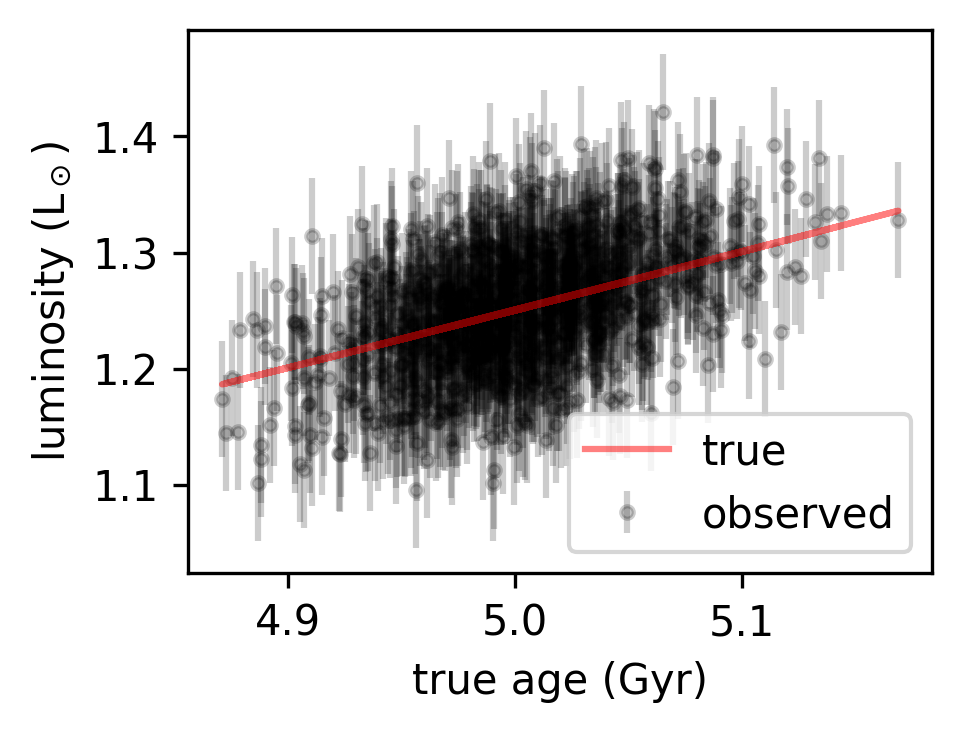
\includegraphics[]{introduction/images/obs_lum.png}
    \caption{Luminosity against true ages of a fake stellar cluster. The true luminosities lie on the red line and the observed luminosities (black) have been artificially scattered by \SI{0.05}{\solarluminosity}.}
    \label{fig:obs_lum}
\end{figure}

If we wished to determine spread of stellar ages in the cluster using the no-pooled model, we might na\"{i}vely calculate a standard deviation from the resulting stellar ages. However, this overestimates the true standard deviation, getting \SI{0.109}{\giga\year} rather than \SI{0.05}{\giga\year}, because it includes the uncertainty in the individual ages. When we model the population mean and spread in the hierarchical model we get $\mu_\tau = \SI{5.002(3)}{\giga\year}$ and $\sigma_\tau = \SI{0.042(7)}{\giga\year}$ which are within $< 2\sigma$ of the truths. Therefore, the hierarachical model is a better way of determining population-level statistics than the traditional no-pooled model.

Both models can accurately determine ages, but the hierarchical model returns more precise ages, assuming our prior assumptions are true. Figure \ref{fig:zscore} shows that the $z$-score for ages from both models match a normal distribution with a mean of 0 and standard deviation of 1, indicating the individual stellar ages and uncertainties are accurate. However, the partially pooled model produces more than doubly precise ages, as shown in Figure \ref{fig:age_unc}, because the model takes into account the population mean and spread as hyper-parameters. The reduced scatter on stellar ages is also reflected in the top-left plot of Figure \ref{fig:zscore}.

\begin{figure}[t]
    \centering
    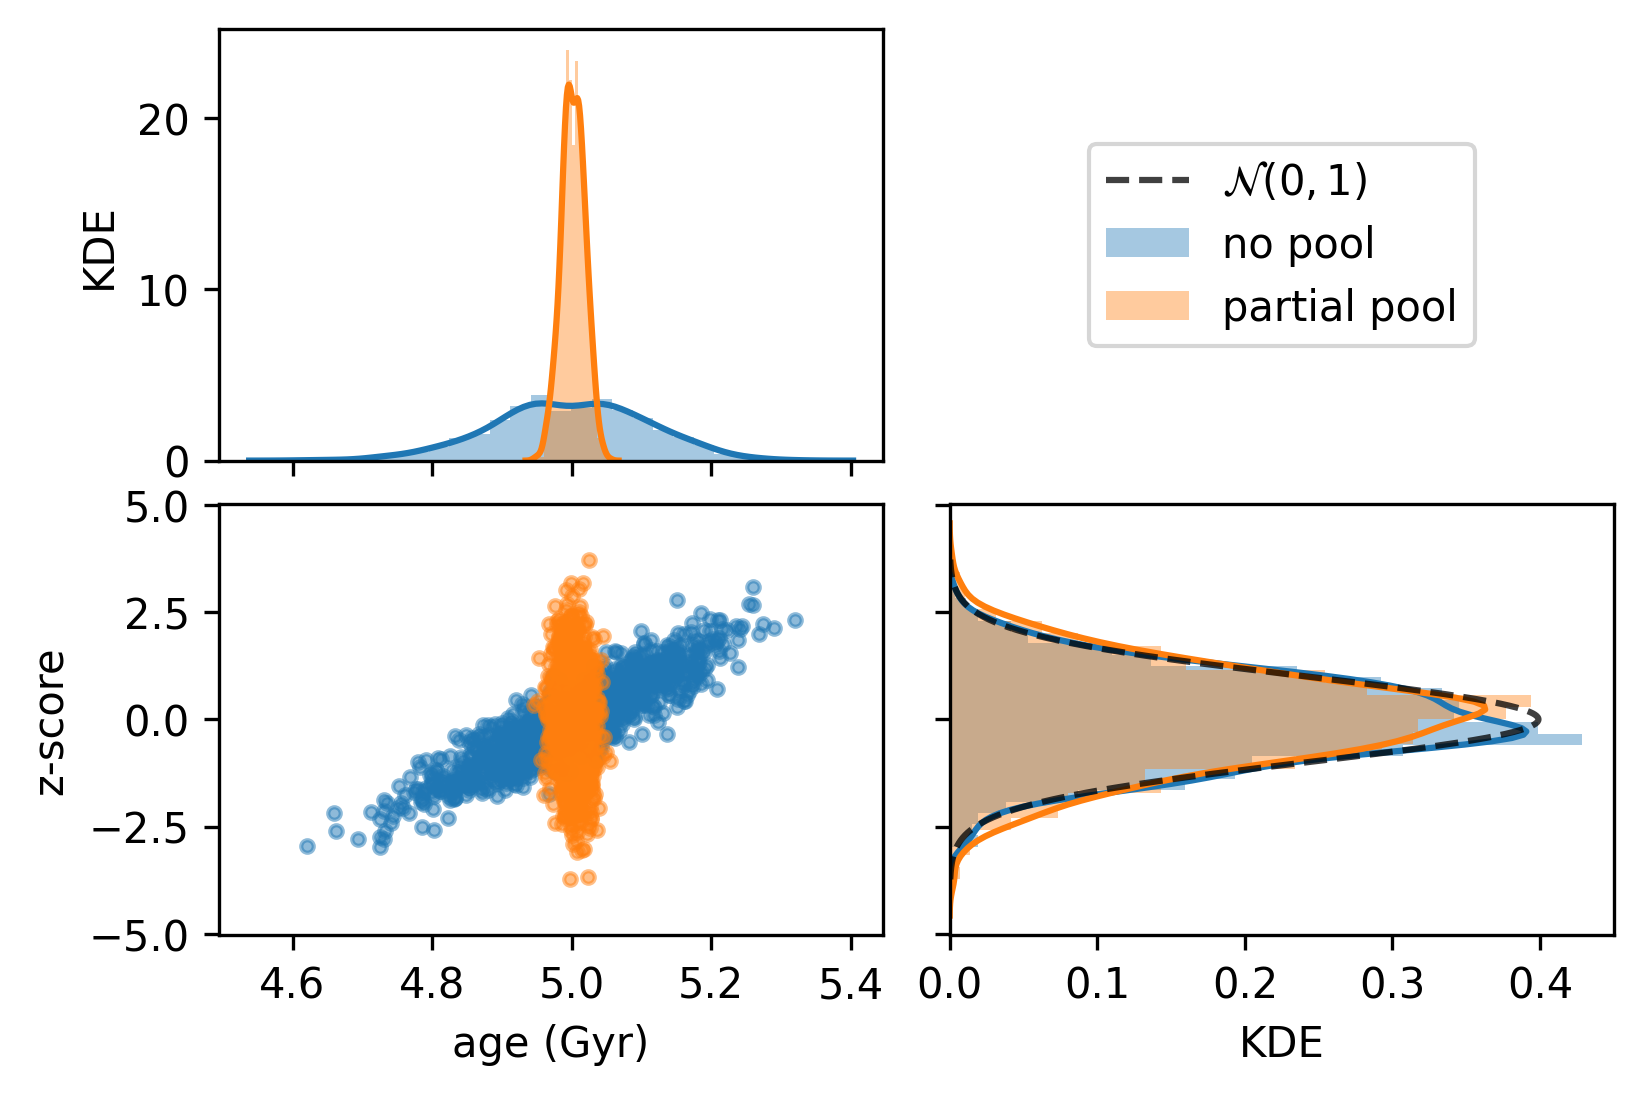
\includegraphics[]{introduction/images/age_z_score.png}
    \caption{The $z$-score, $(\bar{\tau} - \tau_\mathrm{true}) / s_\tau$, where $\bar{\tau}$ and $s_\tau$ are the respective sample mean and standard deviation of the posterior ages from each of the no- and partially-pooled models.}
    \label{fig:zscore}
\end{figure}

\begin{figure}[t]
    \centering
    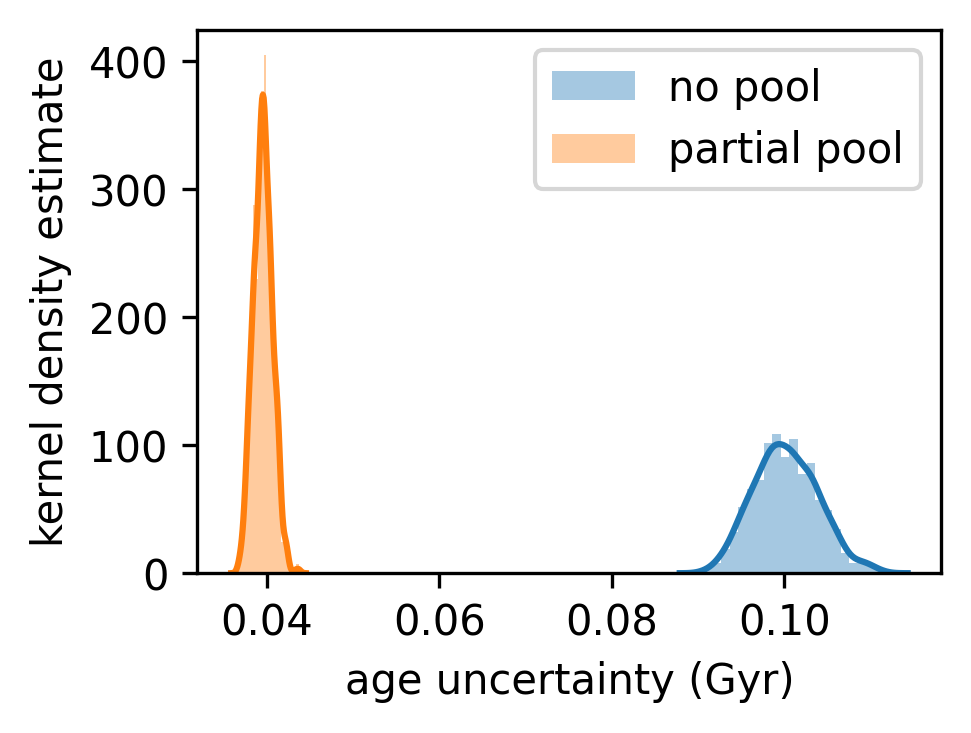
\includegraphics[]{introduction/images/age_uncertainties.png}
    \caption{Standard deviations, $s_\tau$ of the age posteriors from both the no- and partially-pooled models.}
    \label{fig:age_unc}
\end{figure}

If we wish to improve the precision of fundamental stellar parameters, using hierarchical models to encode our prior knowledge is essential. However, modelling stars is not as simple, nor analytical as in the example above. Before we can statistically model a population of stars, we must have a way of generating stellar observables from fundamental parameters such as age and mass. In the next section, I give an overview of how we numerically model stellar observables and why traditional methods pose new problems when adapting the above model.

\section{Modelling a Star}\label{sec:models}

Modelling a star is a complicated process with no simple law which describes the evolution of measurable quantities as a function of its age and initial bulk properties. Following the development of quantum theories of ionization and radiation, the theory of the stellar interior was able to progress from the assumption that stars were a ball of uniform, ideal gas \citet{Eddington1926}. Stellar structure could be simplified to the combined effects of a few differential equations.

The first is the equation of hydrostatic equilibrium which states that the outward pressure within the star acts to oppose the inward gravitational force. This may be written as,
\begin{equation}
    \frac{\partial P(r)}{\partial r}=-\frac{G \rho(r) m(r)}{r^{2}},\label{eq:hydroeq}
\end{equation}
where $P(r)$ is the pressure at a given radius $r$ within the star, $G$ is the gravitational constant, $\rho(r)$ is the density at $r$ and $m(r)$ is the mass contained within $r$. Combined with equations for the conservation of mass, energy loss and internal energy transport, we have can describe the structure of a star.

Integrating Equation \ref{eq:hydroeq} with respect to radius from the centre to the boundary $R$ (where $P(R)=0$) leads to the virial theorem,
\begin{equation}
    \Omega = - 3(\gamma - 1) U,
\end{equation}
where $\Omega$ is the gravitational potential energy of the star, $\gamma$ is the adiabatic exponent which related the pressure of the star to the internal energy density, $u$, $P = (\gamma - 1) u$ assuming an ideal gas, and $U$ is the total internal energy of the star. We show the virial theorem here to demonstrate that if a star contracts, its potential energy decreases which in tern increases its internal energy and flux at the surface.

Internal energy transport within a star is either radiative, convective, or conductive in the case of white drawfs and neutron stars \citep{Yakovlev.Urpin1980}. Energy transportation is important when modelling stars. However, convective energy transfer is notoriously difficult to calculate. When solving for the evolution of stellar structure, we often use approximations of convection such as the mixing-length-theory \citep{Bohm-Vitense1958, Gough1977}. The mixing-length theory characterises the typical distance over which a blob of stellar material moves before dispersing as the fraction $\alpha_\mathrm{mlt}$ of the pressure scale height $H_P = -P (\dd r / \dd P)$, where $\alpha_\mathrm{mlt}$ is of order unity. Since the mixing-length theory is an approximation of convection, its accuracy varies between stellar models and as such the value of $\alpha_\mathrm{mlt}$ is often calibrated to the Sun. However, studies of 2D \citep{Ludwig.Freytag.ea1999} and 3D \citep{Trampedach.Stein.ea2014} hydrodynamical simulations calibrated $\alpha_\mathrm{mlt}$ in the range \numrange{1.5}{2.5} for different stars similar to the Sun.

When a star of similar mass to the Sun (\SIrange{0.8}{1.2}{\solarmass}) begins its life, the conditions in its centre quickly become a high enough temperature and pressure to fuse hydrogen. We call this evolutionary phase the zero-age main sequence (ZAMS). Throughout its main sequence (MS) lifetime, it burns hydrogen to produce helium via the proton-proton (p-p) chain reaction,
\begin{equation}
    4^{1} \mathrm{H}^{+} \rightarrow  {}^{4}\mathrm{He}^{2+}+2 \mathrm{e}^{+}+2 \nu_\mathrm{e}.
\end{equation}
Stars in this mass range typically burn hydrogen in a radiative core surrounded by a convective envelope. Radiative and convective regions are described by the dominant process of energy transport in the region.

Figure \ref{fig:track} shows the evolutionary tracks near-solar-mass stars on a Hertzsprung-Russell diagram (HRD). As a star evolves through the MS, where it is commonly referred to as as \emph{dwarf}, the mean molecular weight of its core increase as hydrogen is being converted to helium. Thus, the core contracts and heats up in accordance with the virial theorem, increasing the nuclear reaction rate and photon flux (or luminosity, $L$) of the star. Towards the end of the MS lifetime, the convective envelope expands, cooling the temperature at the surface of the star (effective temperature, $T_\mathrm{eff}$). Once the star has extinguished available hydrogen in the core, its luminosity decreases and the core contracts because it is no longer supported by nuclear burning. In turn, the convective envelope continues to expand and the effective temperature of the star decreases, while the temperature near the contracting core increases. During this phase, the growing star is often refered to as a \emph{subgiant}. Once conditions in a shell at the boundary of the core are sufficient, hydrogen begins to fuse once more, increasing the luminosity of the star as it evolves from a \emph{subgiant} into a \emph{red giant}

\begin{figure}[ht]
    \centering
    \includegraphics{../kepler-dwarfs/paper/figures/context_tracks.png}
    \caption{A series of stellar evolutionary tracks plot on a Hertzsprung-Russell diagram, starting at the ZAMS and evolved through the MS (black line) to the post MS (dashed black line) until the stellar surface gravity $\log g=3.6$.}
    \label{fig:track}
\end{figure}

Today, we are able to evolve stars to predict their surface quantities such as $L$ and $T_\mathrm{eff}$ using stellar evolutionary codes. Early development of such codes began in the 1960s \citep[see e.g.][]{Kippenhahn.Weigert.ea1967}. Later, stellar models were being computed in large ranges of masses and chemical composition to fit isochrones (tracks at a constant age) to observations of Galactic open clusters \citep{Vandenberg1985}. Today, there are many codes available for scientists to evolve stellar models. In the case of 1D, non-rotating models, there are for example: ASTEC \citep{Christensen-Dalsgaard2008}, CESAM2k \citep{Morel.Lebreton2008}, GARSTEC \citep{Weiss.Schlattl2008} and MESA \citep{Paxton.Bildsten.ea2011}. For 2D and 3D hydrodynamics, current codes include: MUSIC \citep{Baraffe.Pratt.ea2017} for better modelling of convective mixing and 2DStars \citep{Halabi.Izzard.ea2017} to model rotating stars. Other 2D and 3D codes also exist for modelling short-timescale events such as rapidly rotation in stars \citep{Roxburgh2004}.

In this work, we use an open-source 1D stellar evolutionary code called the Modules for Experiments in Stellar Astrophysics \citep[MESA;][]{Paxton.Bildsten.ea2011}. The code evolves a star given a set of initial conditions over dynamically assigned time steps, producing models for the internal stellar structure and a summary of the state of the star at each step. It achieves this by dividing a 1D slice of the star into a mesh of points at which it numerically integrates the stellar differential equtions. 

Example inputs to MESA include: the mass, $M$, the mixing-length theory parameter, $\alpha_\mathrm{mlt}$, and the fractional composition of hydrogen, helium and other heavy elements characterised by the $X$, $Y$ and $Z$ respectively where $X+Y+Z=1$. If the macroscopic diffusion of heavy elements is considered, the chemical composition at the surface of the star will change with time.

\section{Asteroseismology of Solar-Like Oscillators}\label{sec:seismo}

For over a century, we have been able to map stars based on their photometric magnitude and spectroscopic colour with HRDs. Coupling such observational data with measurements of interstellar distances using parallax, we were able to determine stellar luminosities. The unique structure of early HR diagrams eluded to the idea that stars evolve over time. With the addition of nuclear physics, theories of stellar evolution could be put to the test. However, while we could only observe stellar surface properties, many modelling mysteries would be left unsolved.

Until the last few decades, our understanding of stellar structure has been all but skin deep. In the 1960s, observations of 5-minute brightness fluctuations in the solar photosphere lead to the study of stochastically driven acoustic waves trapped beneath the surface of the Sun \citep{Ulrich1970, Ando.Osaki1975}. Later named helioseismology \citep{Deubner.Gough1984}, the study of oscillation modes allowed for further insights into the solar interior, such as rotation \citep{Deubner.Ulrich.ea1979} and solar neutrino production \citep{Bahcall.Ulrich1988}. In tandem with this research was the emergence of asteroseismology -- the study of stars through their oscillation frequencies \citep{Christensen-Dalsgaard1984}. Asteroseismolgy has since been used to improve inference on the fundamental properties of stars \citep[see, e.g.][]{Ulrich1986, Soderblom2010, SilvaAguirre.Davies.ea2015}.

Solar-like oscillators are stars which typical exhibit two kinds of standing waves: acoustic oscillation modes (or p modes) excited stochastically by convection in their outer layers and restored by pressure gradients, and internal gravity waves (or g modes) which are controlled by buoyancy. This work focuses on main sequence stars for which p modes are only present in their spectra. Hence, in this section I will summarise the theory behind acoustic waves present in main sequence stars.

The theory which predicts the locations of the asteroseismic oscillation modes has its roots in the spherical harmonic oscillator. The eigenfrequencies, $\nu_{nlm}$ are categorised into modes of radial order, $n$, angular degree, $l$ and azimuthal order, $m$. The radial order represents the number of standing wave nodes. Figure \ref{fig:modes} shows spherical oscillation modes for different $l$ and $m$. Small changes in stellar radius manifest as small changes in luminosity, arising from the principle of hydrostatic equilibrium. If we imagine the combination of such oscillations when viewing a star as a point source, we can imagine how higher $l$ would be harder to detect due to cancellation across the stellar surface. Typically, we are able to resolve $l \lesssim 3$ in the frequency spectra of stars for which we are unable to resolve the surface.

\begin{figure}[ht]
    \begin{subfigure}[b]{0.2\linewidth}
        
\includegraphics[width=\linewidth]{introduction/images/0_0.png}
        \caption*{$l=0,\,m=0$}
    \end{subfigure}%
    \begin{subfigure}[b]{0.2\linewidth}
        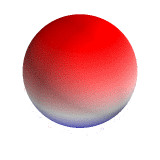
\includegraphics[width=\linewidth]{introduction/images/1_0.png}
        \caption*{$l=1,\,m=0$}
    \end{subfigure}%
    \begin{subfigure}[b]{0.2\linewidth}
        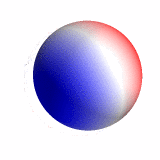
\includegraphics[width=\linewidth]{introduction/images/1_1.png}
        \caption*{$l=1,\,m=1$}
    \end{subfigure}%
    \begin{subfigure}[b]{0.2\linewidth}
        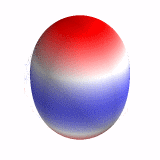
\includegraphics[width=\linewidth]{introduction/images/2_0.png}
        \caption*{$l=2,\,m=0$}
    \end{subfigure}%
    \begin{subfigure}[b]{0.2\linewidth}
        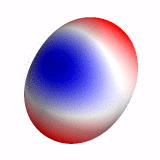
\includegraphics[width=\linewidth]{introduction/images/2_1.png}
        \caption*{$l=2,\,m=1$}
    \end{subfigure}

    \begin{subfigure}[b]{0.2\linewidth}
        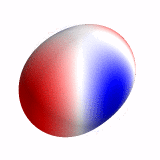
\includegraphics[width=\linewidth]{introduction/images/2_2.png}
        \caption*{$l=2,\,m=2$}
    \end{subfigure}%
    \begin{subfigure}[b]{0.2\linewidth}
        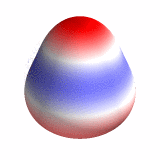
\includegraphics[width=\linewidth]{introduction/images/3_0.png}
        \caption*{$l=3,\,m=0$}
    \end{subfigure}%
    \begin{subfigure}[b]{0.2\linewidth}
        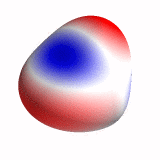
\includegraphics[width=\linewidth]{introduction/images/3_1.png}
        \caption*{$l=3,\,m=1$}
    \end{subfigure}%
    \begin{subfigure}[b]{0.2\linewidth}
        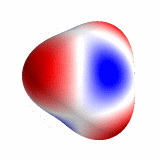
\includegraphics[width=\linewidth]{introduction/images/3_2.png}
        \caption*{$l=3,\,m=2$}
    \end{subfigure}%
    \begin{subfigure}[b]{0.2\linewidth}
        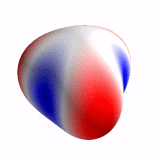
\includegraphics[width=\linewidth]{introduction/images/3_3.png}
        \caption*{$l=3,\,m=3$}
    \end{subfigure}
    \caption{Spherical harmonic modes of oscillation for various combinations of angular degree ($l$) and azimuthal order ($m$).}
    \label{fig:modes}
\end{figure}

Figure \ref{fig:waves} shows the paths of wave fronts travelling through the stellar interior at difference angular degree $l$. The waves curve due to the changing sound speed profile inside the star. We can see how waves with difference $l$ probe different depths of the stellar interior. In the case of the Sun, where modes of high $l$ are able to be resolved, this has allowed us to uncover its density profile \citep{}.

\begin{figure}[ht]
    \centering
    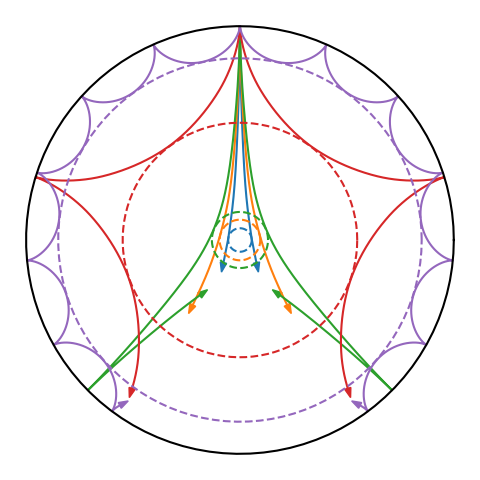
\includegraphics[width=.5\linewidth]{introduction/images/seismo_wavefronts.png}
    \caption{The asteroseismic wave fronts in a typical stellar interior. The blue, orange, green, red and purple lines represent the paths of oscillations with angular degree, $l=1,2,3,25,75$ respectively. The dashed lines represent the depth probed by each mode.}
    \label{fig:waves}
\end{figure}

We characterise the first three angular degrees as radial, $l=0$, dipolar, $l=1$ and quadrupoloar, $l=2$ modes. Observable p modes in solar-like oscillators are typically at high $n$ and low $l$, where asymptotic theory may be applied, $l/n \rightarrow 0$ \citep{Tassoul1980}. Therefore, to first order in $\Delta\nu$, we can approximate the frequency for a given as follows \citep{Christensen-Dalsgaard1984},
%
\begin{equation}
    \nu_{nl} \simeq \Delta \nu\left(n+ \frac{l}{2} + \epsilon\right)\label{eq:seis}
\end{equation}
%
where,
%
\begin{equation}
    \Delta \nu = \left(2 \int_{0}^{R} \frac{\mathrm{d} r}{c(r)}\right)^{-1}
    \label{eq:dnu}
\end{equation}
%
is proportional to the inverse of the sound travel time over the stellar diameter, $2R$ where the speed of sound $c$ is a function of stellar radii. The large frequency separation, $\Delta\nu$ is approximately the frequency difference between consecutive modes of the same $l$. Equation \ref{eq:seis} also implies that consecutive modes of odd and even degree should be separated by $\sim \Delta \nu / 2$. Second-order deviations from Equation \ref{eq:seis} can be shown to describe the small frequency spacing, $\delta \nu_{l\,l+2}$. In other words, we expect to find even and odd modes in $l$ to be found clustered together. In practice, as shown in Section \ref{sec:astero-obs}, we find pairs of radial and quadrupolar modes separated by $\sim \Delta\nu$ and dipolar modes in between them.

% From Equation \ref{eq:dnu}, one can show by substitution of the speed of sound in a gas, that the average large frequency separation, $\langle \Delta \nu \rangle$ scales with the average stellar density, $\langle\rho\rangle$ \citep{Ulrich1986},
% %
% \begin{equation}
%     \left\langle\Delta \nu_{n l}\right\rangle \propto \langle\rho\rangle^{1 / 2}.
% \end{equation}
% %

We detect exceited oscillation modes in an excess of power centred on the frequency at maximum power, $\nu_\mathrm{max}$. By characterising the behaviour of the waves close to the stellar surface, it can be shown that $\nu_\mathrm{max} \propto g T_\mathrm{eff}$ where $g$ is the surface gravity of the star \citep{Kjeldsen.Bedding1995}.

We can determine theoretical oscillation modes by solving for the stellar profiles produced in the evolutionary models discussed in Section \ref{sec:models}. One such code build to predict oscillation modes for a given stellar structure is GYRE \citep{Townsend.Teitler2013}. 

\section{Sampling Stellar Models}

Stellar evolution and astrometric models can predict observables given the age and initial conditions (e.g. mass, chemical composition and other model physics) for a given star. To implement the HBM described in Section \ref{sec:hbm} we need a way to generate predictions from the stellar models. There are generally two methods for achieving this: produced a discrete grid of models and evaluate the likelihood at each point or interpolate a grid of models and continuously sample an approximation of the grid. It is difficult to implement an HBM using either of these methods, because we need it to scale well with input dimensions and number of stars in a population.

Grid-based modelling involves producing a large grid of stellar models with a range of input parameters. Then, the likelihood that a star is described by a point on the grid may be evaluated \citep[see e.g. BASTA][]{SilvaAguirre.Davies.ea2015}. However, using a discrete grid can lead to inaccurate model posteriors limited by the grid spacing and computing finer grids is more computationally expensive.

Alternatively, we can interpolate the grid of models. This is common in the isochrone fitting method \citep{}. Here, a grid of models in 3 dimensions (mass, metallicity and age) may be easily interpolated to produce an approximation of the stellar models, continuously mapping inputs to observables. However, interpolation does not scale well with input dimensionality and size of the grid. In order to take full advantage of the HBM, we need the flexibility to expand the input dimensions to encompass extra model physics such as the mixing-length theory parameter, $\alpha_\mathrm{mlt}$. We need a faster way of approximating the grid of stellar models, which scales well with dimensions.

One alternative to interpolation is to use machine learning. We can train an artificial neural network on the grid of models. This is the method used in Chapter \ref{ch:paper} and is explained in more detail in the attached paper (Appendix \ref{apx:paper}). In summary, the neural network is made up of many layers of trainable weights which are optimised to minimise the error between predictions and the training data. Advantageously, it is easy to evaluate the gradient of the likelihood of neural network predictions, because said gradient is required to optimise the weights. Therefore, approximating the models this way allows us to sample the posterior of the HBM using modern algorithms such as Hamiltonian Monte Carlo (HMC) \citep[see e.g. the No-U-Turn Sampler][]{Homan.Gelman2014}.

\section{Observing Stars}

In this section, we briefly recall the fundamentals of observational astronomy. We first describe a method for determining luminosity from photometric and astrometric measurements. Then, we show how spectroscopy can determine the chemical composition and temperature at the surface of a star. Finally, we show how we determine the asteroseismic oscillation modes from photometric time series measurements of a solar-like oscillator.

\subsection{Photometry \& Astrometry}

Photometry is the measure of photon flux from an object. In stellar astronomy, we can use photometry to determine the luminosity, $L$, of a star and measure short-timescale variations in flux due to stellar activity and pulsations. We measure the flux from an object in a series of passbands. For example, if we measure the photmetric flux, $F$, from a star in the blue ($B$) and visual ($V$) bands then we which we can determine its apparent visual magnitude, $m_V$,
\begin{equation}
    m_V = - 2.5 \log(\frac{F_V}{F_{V,0}}),
\end{equation}
where $F_{V,0}$ is the reference flux at a magnitude of zero, and its colour, $m_B - m_V$.

Astrometry is the measure of the position and movement of a star across the sky. We can measure the position of a star against a distant background throughout the year to determine its parallax ($\varpi$) -- the apparent difference in angular position of a star in the sky between observations separated by 1 astronomical unit (AU\footnote{The average distance between the Earth and the Sun, $\SI{1}{\mathrm{AU}} \approx \SI{1.5e8}{\kilo\meter}$.}). We can then derive the distance, $d$ to the star assuming the small-angle formula, $d \approx 1/\varpi$. We typically measure $\varpi$ in arc seconds (`''' or `as'), which yields a distance in parsecs (pc) -- the distance from the Sun to an object which has moved \SI{1}{''} over a baseline of \SI{1}{AU}.

If we wish to determine the luminosity of a star (photometric flux at the stellar surface), we need the distance to the star which we can determine using astrometry. We first calibrate the absolute magnitude, $\mathcal{M}$ of the star to get its flux at a distance of \SI{10}{pc}. For example, in the $V$-band,
\begin{equation}
    \mathcal{M}_V = m_V - 5 \log(d) + 5 + A_V,
\end{equation}
where $A_V$ is the extinction -- an estimate of the light absorbed by interstellar dust between the star and the observer. However, to get to luminosity, we need the total flux across the entire electromagnetic spectrum. We can estimate this by calculating a bolometric correction ($BC$) which can be empirically determined or modelled by the surface properties of the star. The bolometric magnitude, $\mathcal{M}_\mathrm{bol}$,
\begin{equation}
    \mathcal{M}_\mathrm{bol} = \mathcal{M}_V - BC,
\end{equation}
is related to the luminosity of the star,
\begin{equation}
    \frac{L}{\mathrm{L}_{\odot}}=10^{\frac{2}{5}\cdot\left(\mathcal{M}_{\mathrm{bol}, \odot}-\mathcal{M}_{\mathrm{bol}}\right)},
\end{equation}
in terms of the solar luminosity, \si{\solarluminosity}.

\subsection{Spectroscopy}

Stellar spectroscopy is the measure and analysis of the electromagnetic spectra of stars. We can use this to determine the abundance of elements in the stellar surface to the effective temperature, $T_\mathrm{eff}$.

The abundances of elements are typically reported as the ratio of the element to a readily abundant element. For example, the iron abundance is given as $[\mathrm{Fe/H}]$ and is the logarithmic difference between the fractional abundance in the stellar spectra with that of the Sun. We write the metallicity as the relative abundance of all elements except for H and He,
\begin{equation}
    [\mathrm{M/H}] = \log(Z/X) - \log(Z/X)_\odot,
\end{equation}
where $(Z/X)_\odot$ is the relative abundance of heavy-elements to hydrogen in the Sun. The solar value has been revised downward over recent years but is $(Z/X)_\odot \approx 0.02$ \citep{Grevesse.Sauval1998, Asplund.Grevesse.ea2005, Asplund.Grevesse.ea2009}

The stellar electromagnetic spectrum can also be used to determine its surface temperature, $T_\mathrm{eff}$ which is fundamentally related to the luminosity of a star of radius $R$, $L \propto R^2T_\mathrm{eff}^4$. We can determine the luminosity using Wein's law,
\begin{equation}
    \lambda_\mathrm{max} T_\mathrm{eff} \approx \SI{2.9e-3}{\meter\kelvin},
\end{equation}
where $\lambda_\mathrm{max}$ is the wavelength at maximum power.

We have shown the basic theory behind determining temperature and abundances from spectroscopy, but there are a whole lot more to the process which goes beyond the scope of this work. A continuously updated source of abundances and parameters is the APOGEE stellar parameters and chemical abundances pipeline \citep[ASPCAP;][]{GarciaPerez.AllendePrieto.ea2016} of the Sloan Digital Sky Survey \citep[SDSS;][]{Blanton.Bershady.ea2017}.

\subsection{Detecting Asteroseismic Oscillation Modes}\label{sec:astero-obs}

We can measure the asteroseismic frequencies to higher precision than traditional stellar parameters such as $L$ and $T_\mathrm{eff}$, allowing for more precise comparison with stellar models.

In order to characterise the asteroseismic oscillations of a star, we need measurements of its photometric time series. Several missions from \emph{Kepler} \citep{Borucki.Koch.ea2010} to more recently, TESS \citep{Ricker.Winn.ea2015} have provided time series data. We can extract the frequency-power spectrum from the time series using the Lomb-Scargle method \citep{Lomb1976, Scargle1982}. Figure \ref{fig:spec} shows an example of an asteroseismic power spectrum for TIC 38828538 (Buldgen et al. in preparation). There is a power excess at around \SI{200}{\micro\hertz} which contains the excited oscillation modes. These are a series of peaks within the power element which correspond to frequencies, $\nu_{nl}$ of different radial order ($n$) and angular degree ($l$).

\begin{figure}
    \centering
    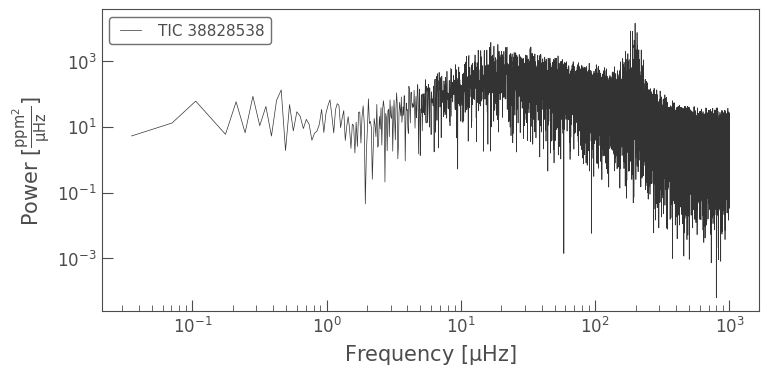
\includegraphics[width=0.8\linewidth]{introduction/images/sprectrum.png}
    \caption{The frequency-power spectrum for a red giant star.}
    \label{fig:spec}
\end{figure}

Figure \ref{fig:peakbag} shows the signal-to-noise (SNR; total power divided by an estimate of the background noise) spectrum for the star around the frequency of maximum power, $\nu_\mathrm{max} \approx \SI{200}{\micro\hertz}$. We can see that  

\begin{figure}
    \centering
    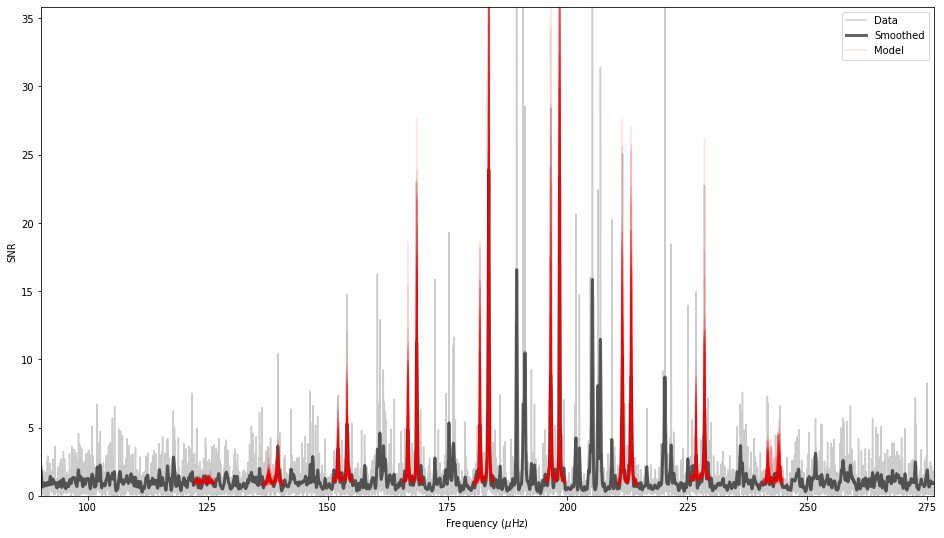
\includegraphics[width=0.8\linewidth]{introduction/images/peakbag.png}
    \caption{The signal-to-noise (SNR) power spectrum for a red giant star with 100 random samples from the posterior locations of the $l=0,2$ oscillation mode pairs.}
    \label{fig:peakbag}
\end{figure}

There are several methods which exist to extract the radial and quadrupolar ($l=0, 2$) oscillation modes from the asteroseismic power spectra \citep[see e.g.][]{Mosser.Belkacem.ea2011, Appourchaux.Chaplin.ea2012, Davies.Aguirre.ea2016}. In this work, we use the Python package \texttt{PBjam} (Nielsen et al. in preparation) to demonstrate one such method.

\begin{figure}
    \centering
    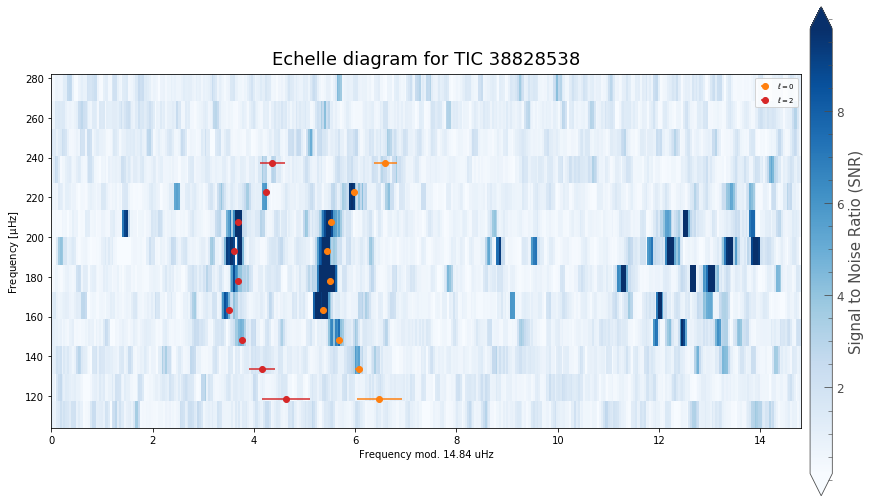
\includegraphics[width=0.8\linewidth]{introduction/images/echelle.png}
    \caption{An echelle diagram for a red giant star with the locations of the radial ($l=0$) and quadrupolar ($l=2$) oscillation modes.}
    \label{fig:echelle}
\end{figure}
